\chapter{Conception et architecture}

\section{Introduction}
Ce chapitre explique comment le système est construit. Nous justifions d'abord les technologies retenues, puis nous décrivons l'architecture logique, l'architecture physique et le modèle de données. Nous détaillons enfin le scénario dont la logique est la plus fine, l'audit asynchrone d'un site, au moyen de diagrammes de séquence. Les diagrammes UML suivent la notation standard \cite{omguml}.

\section{Choix technologiques}
Le cahier des charges recommandait une API en Python, une interface React et une base relationnelle. Notre pile (\cref{fig-stack}) suit ces recommandations ; le \cref{tab-techno} justifie chaque choix.

\fig[0.9]{figures/architecture/stack_logos.jpeg}{Principales technologies de \xapp}{fig-stack}
\source{schéma réalisé pour la présentation du projet}

\begin{table}[htbp]
\centering
\small
\caption{Technologies retenues et justification}\label{tab-techno}
\begin{tabularx}{\textwidth}{@{}p{2.6cm}p{3.6cm}X@{}}
\toprule
\textbf{Couche} & \textbf{Technologie} & \textbf{Raison du choix}\\
\midrule
Interface & Next.js~16, React~19, TypeScript, Tailwind CSS \cite{nextjsdocs,reactdocs} & Routage par fichiers (App Router), rendu serveur des pages publiques utile au référencement de la plateforme elle-même, typage, écosystème riche (Recharts, Framer Motion)\\
Internationalisation & next-intl & Trois langues (FR, EN, AR) avec bascule \gls{rtl} pour l'arabe, messages centralisés en JSON\\
API & Python, FastAPI, Uvicorn \cite{fastapidocs} & Python est le langage naturel de l'analyse HTML (BeautifulSoup) et des SDK d'IA ; FastAPI est asynchrone, valide les entrées par Pydantic et génère la documentation Swagger \cite{fielding2000rest}\\
Accès aux données & SQLAlchemy \cite{sqlalchemydocs} & \gls{orm} mature ; le même code fonctionne sur SQLite en développement et PostgreSQL en production via \code{DATABASE\_URL}\\
Base de données & PostgreSQL (production), SQLite (développement) \cite{postgresqldocs} & Intégrité référentielle pour les crédits et paiements, colonnes texte pour stocker les résultats d'audit en JSON\\
Crawl et analyse & aiohttp, httpx, BeautifulSoup4, lxml & Requêtes HTTP concurrentes et asynchrones, analyse robuste de HTML imparfait\\
Performance & Google PageSpeed Insights API \cite{pagespeeddocs} & Core Web Vitals mesurés par Google (\gls{lcp}, \gls{cls}, \gls{inp}) plutôt que recalculés\\
Intelligence artificielle & OpenAI (GPT-4o, GPT-4o-mini), Groq \cite{openaidocs,groqdocs} & OpenAI pour le plan d'action et la présence dans ChatGPT ; Groq pour Jannet et la transcription (Whisper), rapide et à faible coût\\
PDF & ReportLab & Génération côté serveur de rapports et plans d'action signés\\
Paiement & Flouci \cite{flouci} & Passerelle tunisienne permettant de payer en dinars\\
Hébergement & VPS Ubuntu, Nginx, systemd, PM2, GitHub Actions \cite{nginxdocs,pm2docs} & Contrôle complet de l'environnement, coût fixe, déploiement automatique à chaque push\\
\bottomrule
\end{tabularx}
\end{table}

\subsection{Pourquoi deux langages ?}
Le choix d'un front en TypeScript et d'une API en Python impose deux écosystèmes. Nous l'avons assumé parce que chaque côté profite de son meilleur outillage : l'analyse de pages, le calcul des scores et les appels aux modèles de langage sont plus simples en Python, tandis que Next.js offre un rendu serveur et une internationalisation que les cadriciels Python n'égalent pas. Le contrat entre les deux est une API REST en JSON, authentifiée par jeton, documentée automatiquement par FastAPI.

\subsection{Pourquoi pas de file de messages ?}
Un audit Pro dure de quelques dizaines de secondes à plusieurs minutes, bien au-delà de la centaine de secondes qu'autorise le proxy Cloudflare placé devant le serveur. La solution classique serait une file de messages (Redis et Celery). Nous avons préféré un exécuteur intégré à FastAPI : une boucle asyncio, lancée au démarrage, qui traite les jobs enregistrés en base un par un. Ce choix évite un service supplémentaire sur un serveur unique ; il limite en contrepartie le débit à un audit lourd à la fois, ce que nous discutons au chapitre~\ref{chap-deploiement}.

\section{Architecture logique}
L'application suit une architecture client-serveur découplée en couches (\cref{fig-archi-logique}).

\begin{figure}[htbp]
\centering
\begin{tikzpicture}[every node/.style={font=\small},
  box/.style={draw,rounded corners,fill=grisclair,minimum width=3.4cm,minimum height=0.9cm,align=center},
  ext/.style={draw,rounded corners,fill=jauneaw!25,minimum width=2.8cm,minimum height=0.8cm,align=center},
  lab/.style={font=\footnotesize,fill=white,inner sep=1pt},
  arr/.style={-{Stealth[length=2mm]},thick}]
  \node[box] (nav) at (0,0) {Navigateur\\(FR / EN / AR)};
  \node[box] (front) at (0,-2) {Frontend Next.js~16\\React~19, next-intl};
  \node[box,minimum width=5.6cm] (api) at (0,-4.4) {API FastAPI\\auth, audit, ai-visibility, admin,\\jannet, tickets, team-chat\ldots};
  \node[box] (engine) at (-2.3,-6.9) {Moteur d'audit\\(crawl, scoring)};
  \node[box] (runner) at (2.3,-6.9) {Exécuteur\\asynchrone};
  \node[box] (db) at (0,-9) {SQLAlchemy\\PostgreSQL / SQLite};
  \node[ext] (google) at (6.6,-3.2) {PageSpeed, GSC};
  \node[ext] (ia) at (6.6,-4.4) {OpenAI, Groq};
  \node[ext] (pay) at (6.6,-5.6) {Flouci, SMTP};
  \draw[arr] (nav)--node[lab,right=2pt]{HTTPS}(front);
  \draw[arr] (front)--node[lab,left=2pt]{REST + JWT, SSE, WebSocket}(api);
  \draw[arr] (api)--(engine); \draw[arr] (api)--(runner);
  \draw[arr] (engine)--(db); \draw[arr] (runner)--(db);
  \draw[arr] (api.east)--(ia.west); \draw[arr] (api.east)--(google.west); \draw[arr] (api.east)--(pay.west);
\end{tikzpicture}
\caption{Architecture logique en couches}\label{fig-archi-logique}
\end{figure}

\paragraph{Couche présentation (Next.js).} L'interface utilise l'App Router : chaque dossier de \route{app/} correspond à une route (\route{/dashboard/analyse}, \route{/dashboard/ai-visibility}, etc.). Les pages publiques (accueil en trois langues, méthodologie du score, pages légales) bénéficient du rendu serveur. Un client Axios unique (\code{lib/api.ts}) ajoute le jeton à chaque requête et redirige vers la connexion en cas d'erreur 401. Un contexte React (\code{SubscriptionContext}) expose en temps réel le plan, les crédits et les fonctionnalités débloquées, ce qui permet d'afficher ou de verrouiller les menus.

\paragraph{Couche applicative (FastAPI).} Elle est organisée en routeurs par domaine : authentification, administration, audits et visibilité IA (dans \code{main.py}), Jannet, réunion vocale, paiements, export PDF, notifications, messagerie d'équipe et tickets. Plus d'une centaine de routes REST sont exposées ; la liste par domaine figure en annexe. Les dépendances FastAPI (\code{get\_current\_user}, \code{get\_admin\_user}) appliquent l'authentification et les rôles. Un service dédié (\code{services/credit\_service.py}) concentre la logique des crédits.

\paragraph{Moteur d'audit.} Le paquet \code{audit/} est une bibliothèque interne indépendante de l'API : crawl, analyse de page, audits vitrine et e-commerce, score du site complet, PageSpeed, visibilité IA et présence dans les réponses des modèles. Il peut être appelé de façon synchrone (audit de la page d'accueil) ou par l'exécuteur asynchrone (audit Pro).

\paragraph{Couche données.} Dix-huit tables décrivent les entités (\cref{sec-modele-donnees}). Les résultats d'audit, volumineux et de structure variable, sont stockés en JSON dans une colonne texte, à côté des colonnes qui servent aux recherches (score, type, date).

\paragraph{Canaux temps réel.} En plus du REST, deux canaux poussent des données vers le navigateur : un flux \gls{sse} pour afficher progressivement les réponses des moteurs IA, et une connexion WebSocket authentifiée pour les notifications.

\section{Architecture physique et déploiement}
En production, tout tourne sur un unique serveur privé virtuel Ubuntu (\cref{fig-deploiement}). Cloudflare assure le DNS ; Nginx reçoit les requêtes en HTTPS (port~443), termine le chiffrement TLS avec un certificat Let's Encrypt et route les chemins \route{/api}, \route{/auth}, \route{/audit} et \route{/admin} vers l'API (Uvicorn, port~8000, supervisé par systemd), et tout le reste vers le serveur Next.js (port~3000, supervisé par PM2). PostgreSQL tourne sur la même machine et n'est pas exposé à Internet. \todo{indiquer les caractéristiques du VPS (processeur, mémoire, disque), la version d'Ubuntu et de PostgreSQL}

\fig[0.95]{figures/architecture/deploiement.png}{Diagramme de déploiement}{fig-deploiement}
\source{diagramme PlantUML du dépôt (\code{docs/uml/deployment.puml})}

\section{Modèle de données}\label{sec-modele-donnees}
Le diagramme de classes de la \cref{fig-classes} présente les entités principales. Il est présenté sur une page à l'italienne pour rester lisible.

\begin{landscape}
\begin{figure}[p]
  \centering
  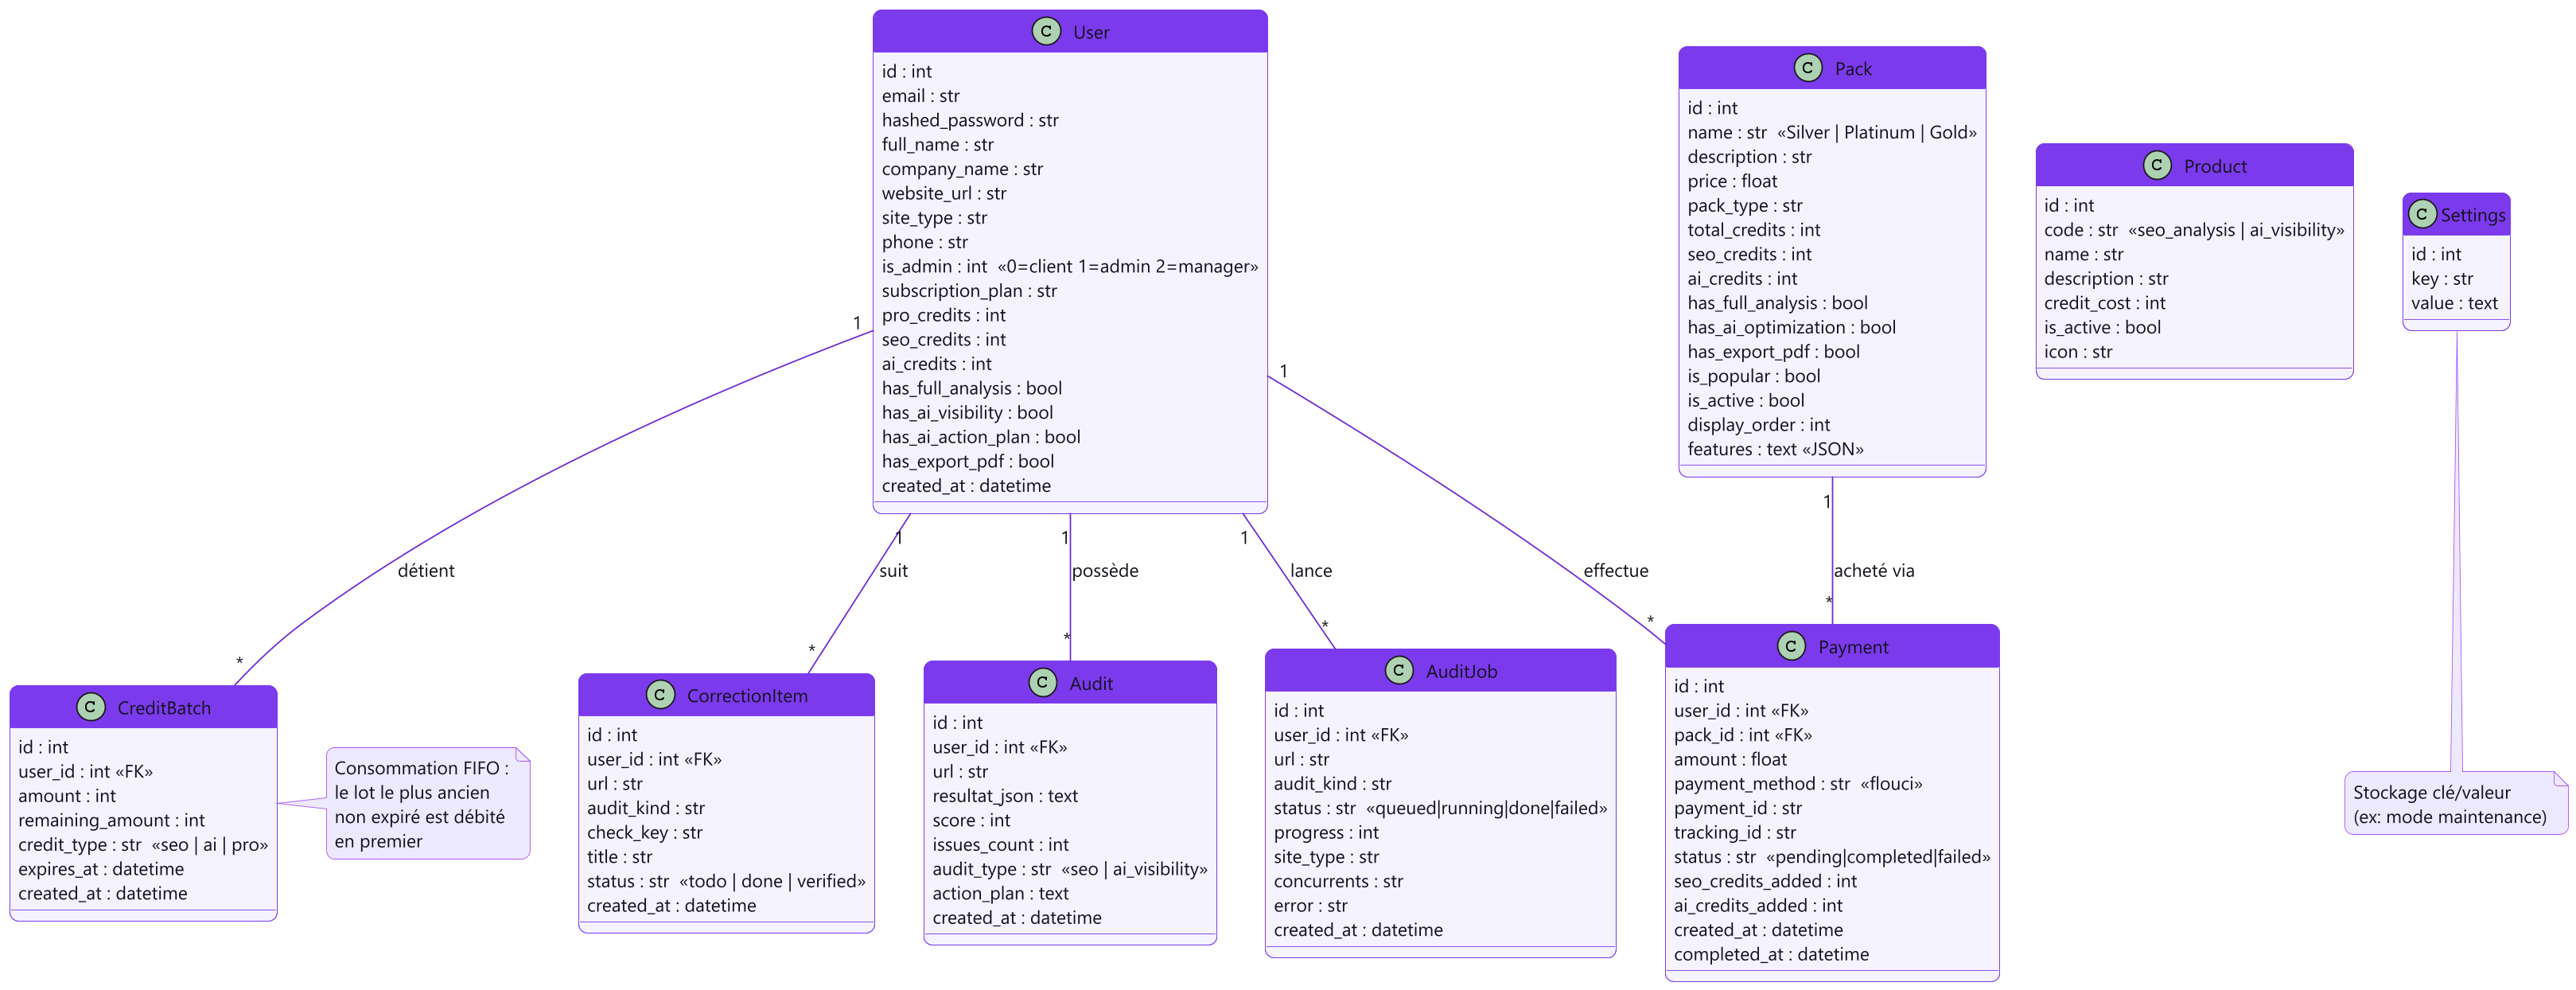
\includegraphics[width=0.96\linewidth,height=0.8\textheight,keepaspectratio]{figures/uml/class_diagram.png}
  \caption{Diagramme de classes (modèles SQLAlchemy principaux)}\label{fig-classes}
\end{figure}
\end{landscape}

\todo{le diagramme de classes ne montre que 9 entités sur 18 ; ajouter les tables de collaboration (tickets, messages, notifications, chat, agent, exports) ou préciser dans la légende qu'il s'agit du cœur métier}

Le \cref{tab-collections} donne le rôle de chaque table.

\begin{table}[htbp]
\centering
\small
\caption{Tables de la base de données et rôle}\label{tab-collections}
\begin{tabularx}{\textwidth}{@{}p{4.2cm}X@{}}
\toprule
\textbf{Table} & \textbf{Rôle}\\
\midrule
\code{users} & Compte, rôle (\code{is\_admin}), plan, soldes de crédits, fonctionnalités débloquées, codes de vérification et de réinitialisation, jeton Search Console\\
\code{audits} & Résultat d'un audit SEO ou IA (JSON), score, nombre de problèmes, plan d'action enregistré\\
\code{audit\_jobs} & Job asynchrone : statut, progression, pages analysées, tranche de pages, crédit utilisé et remboursement\\
\code{correction\_items} & Correction à effectuer : catégorie, gravité, pages concernées, statut, historique\\
\code{credit\_batches} & Lot de crédits avec type, montant restant et date d'expiration\\
\code{packs}, \code{products} & Offres commerciales et coût en crédits de chaque action\\
\code{payments} & Paiements (Flouci), statut, crédits ajoutés\\
\code{exports} & Rapports PDF générés avec leur signature\\
\code{tickets}, \code{ticket\_messages} & Tickets de support et leurs échanges\\
\code{knowledge\_entries} & Base de connaissances de Jannet, alimentée par les tickets résolus\\
\code{agent\_actions} & Journal des actions de l'agent Jannet, avec données d'annulation\\
\code{notifications} & Notifications persistées\\
\code{chat\_channels}, \code{chat\_channel\_members}, \code{chat\_messages} & Messagerie d'équipe : canal général et conversations privées\\
\code{settings} & Paramètres clé/valeur (mode maintenance)\\
\bottomrule
\end{tabularx}
\end{table}

Quelques décisions de modélisation méritent d'être signalées.

\begin{itemize}
  \item \textbf{Crédits en lots.} Le solde affiché sur l'utilisateur n'est qu'un cache ; la vérité est dans \code{credit\_batches}. Chaque achat crée un lot daté, avec une expiration, et la consommation débite d'abord le lot non expiré le plus ancien (\gls{fifo}).
  \item \textbf{Résultats en JSON.} La structure d'un résultat d'audit change selon le type (vitrine, e-commerce, IA) et a évolué au fil des sprints. La stocker en JSON évite une migration à chaque nouvel indicateur.
  \item \textbf{Job distinct de l'audit.} \code{audit\_jobs} décrit l'exécution (file, progression, erreur), \code{audits} le résultat. Un job échoué n'encombre pas l'historique et son crédit peut être remboursé.
  \item \textbf{Corrections identifiées par clé.} Chaque correction porte une clé machine (\code{check\_key}) qui permet à la fois d'éviter les doublons d'un audit à l'autre et de revérifier précisément ce point.
\end{itemize}

\section{Diagrammes de séquence}

\subsection{Audit SEO asynchrone}
Le scénario se découpe en deux phases : le lancement (\cref{fig-seq-audit-1}) et le traitement en arrière-plan avec le suivi de progression (\cref{fig-seq-audit-2}).

\fig[0.95]{figures/uml/sequence_audit_1.png}{Séquence : lancement d'un audit et consommation du crédit}{fig-seq-audit-1}

Au lancement, le client saisit l'adresse de son site. L'API vérifie le jeton, débite un crédit selon la règle FIFO, crée un job à l'état \code{queued} et répond immédiatement avec son identifiant (code~202). L'utilisateur n'attend donc pas la fin du crawl pour récupérer la main.

\fig[0.95]{figures/uml/sequence_audit_2.png}{Séquence : traitement en arrière-plan et suivi de progression}{fig-seq-audit-2}

L'exécuteur récupère le job, le passe à \code{running}, lance le crawl et l'analyse des pages, met à jour la progression en base et enregistre le résultat. Pendant ce temps, le frontend interroge \route{/audit/status/\{job\_id\}} toutes les trois secondes. En cas d'échec ou de dépassement du budget de 600~secondes, le job passe à \code{failed} et le crédit est remboursé.

\section{Conclusion}
L'architecture retenue sépare nettement l'interface, l'API, le moteur d'audit et les données, et isole les traitements longs dans un exécuteur asynchrone. Le chapitre suivant aborde la réalisation, en commençant par le socle commun à tous les modules : les comptes et le contrôle d'accès.
